\documentclass[border=1mm]{standalone}
\usepackage{pgfplots}
\usetikzlibrary{calc}
\pgfplotsset{
    axis lines=middle,
    no markers,
    samples=200,
    grid=both,
    minor grid style={line width=.1pt,draw=gray!50},
    major grid style={line width=.1pt,draw=gray!50},
    enlargelimits={abs=0.5},
    trig format plots=rad,
    every axis plot/.append style={
        line width=0.75pt,
        smooth,
    },
}

\begin{document}
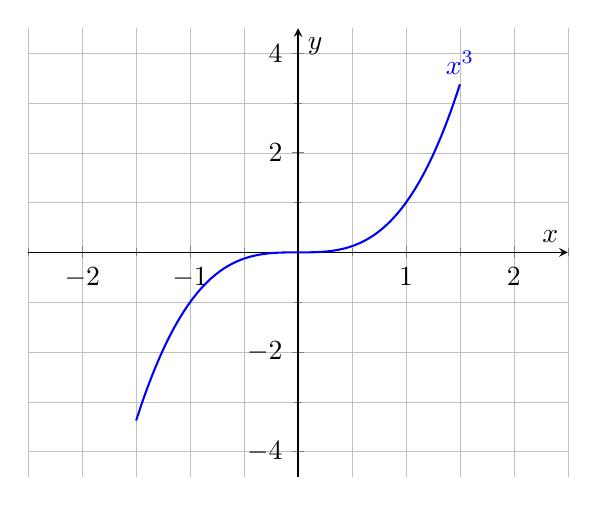
\begin{tikzpicture}
\begin{axis}[
    xlabel=$x$,
    ylabel=$y$,
    domain=-1.5:1.5,
    xmin=-2, xmax=2,
    ymin=-4, ymax=4,
    minor tick num=1,
    restrict y to domain=-10:10
]
    \addplot {x^3} node[above,pos=1] {$x^3$};

\end{axis}
\end{tikzpicture}
\end{document}
